\documentclass[runningheads]{llncs}

\usepackage[utf8]{inputenc}
\usepackage[T1]{fontenc}
\usepackage[spanish,es-tabla]{babel}
\usepackage{graphicx}
\usepackage{booktabs}
\usepackage{amsmath}
\usepackage{url}
\usepackage{xcolor}
\usepackage{amssymb}

\begin{document}

\title{Búsqueda aproximada de vecinos sobre embeddings estáticos y acumulativos para memoria conversacional en diálogos orientados a tareas}

\titlerunning{Búsqueda aproximada de vecinos sobre embeddings conversacionales}

\author{Juan Manuel Fernández\orcidID{0000-0001-9291-3066}}
\authorrunning{J. M. Fernández}

\institute{
\email{jmfernandez@unlu.edu.ar}
}
\maketitle

\begin{abstract}
En los sistemas de diálogo orientado a tareas, la representación del estado conversacional constituye un componente central para la toma de decisiones del agente. Si bien los \textit{embeddings} permiten representar turnos individuales como vectores densos, los diálogos son procesos secuenciales en los que el significado de cada intervención depende del historial acumulado y de su función dentro del flujo conversacional. En este trabajo se estudia la búsqueda aproximada de vecinos sobre \textit{embeddings} estáticos y acumulativos para la recuperación eficiente de situaciones conversacionales en diálogos orientados a tareas.

Para ello, se construyó una colección experimental de 101.021 diálogos completos y 1.000.023 turnos obtenidos a partir de \textit{Dialog2Flow}. Se generaron representaciones mediante dos modelos generales de \textit{sentence embeddings}, \textit{all-MiniLM-L6-v2} y \textit{all-mpnet-base-v2}, y mediante un modelo específico para flujos conversacionales, \textit{dialog2flow-joint-bert-base}. Además, se evaluó una variante acumulativa normalizada sobre cada espacio de representación, con el objetivo de analizar el efecto de incorporar información secuencial del historial. Sobre estas representaciones se evaluaron índices implementados en \textit{FAISS}, incluyendo \textit{IVF}, \textit{HNSW} e \textit{IVFPQ}.

Los experimentos muestran compromisos claros entre precisión, velocidad y memoria: \textit{HNSW} ofrece un balance favorable entre recuperación y eficiencia, mientras que \textit{IVFPQ} reduce sustancialmente la memoria con pérdida de precisión. Además, se incorporó una evaluación semántico-funcional asistida por LLM sobre los vecinos recuperados. Los resultados muestran que la variante acumulativa mejora la recuperación semántico-funcional cuando se aplica sobre el espacio conversacional específico de \textit{Dialog2Flow}, alcanzando los mayores valores de MSS@10 bajo \textit{IVF}, \textit{HNSW} e \textit{IVFPQ}. Esta mejora no se observa de forma equivalente sobre los modelos generales \textit{MiniLM} y \textit{MPNet}.

Estos resultados sugieren que la búsqueda aproximada de vecinos puede funcionar como un componente eficiente de memoria conversacional y que la utilidad de las representaciones acumulativas depende de la geometría del espacio base, especialmente cuando este se encuentra orientado a regularidades de flujos conversacionales.

\keywords{Diálogo orientado a tareas \and Embeddings \and Búsqueda aproximada \and Memoria conversacional \and FAISS \and Dialog2Flow}

\end{abstract}

\section{Introducción}

Los sistemas de diálogo orientados a tareas constituyen un área central dentro de la investigación en procesamiento del lenguaje natural y agentes conversacionales. En este tipo de sistemas, el agente interactúa con el usuario con el objetivo de completar una tarea específica, como reservar un restaurante, buscar información sobre hoteles, solicitar un servicio de transporte o completar una operación sobre un sistema externo. Para ello, el sistema debe interpretar cada intervención del usuario, mantener una representación coherente del estado del diálogo y decidir la acción más adecuada en cada turno de la interacción \cite{young2013pomdp,chen2017survey}.

Una práctica extendida para representar las intervenciones del diálogo consiste en utilizar \textit{embeddings} semánticos, es decir, representaciones vectoriales densas generadas a partir de modelos de lenguaje. En este enfoque, cada turno del diálogo se codifica de manera independiente mediante un vector que captura información semántica del enunciado. Este tipo de representaciones permite aplicar técnicas de recuperación vectorial, clasificación o \textit{clustering} sobre grandes colecciones de interacciones conversacionales \cite{devlin2019bert,reimers2019sentencebert}.

Sin embargo, los diálogos son procesos intrínsecamente secuenciales en los que el significado de cada intervención depende del contexto acumulado de la conversación. En los sistemas de diálogo orientado a tareas, esta dependencia contextual se formaliza habitualmente mediante nociones como estado del diálogo, estado de creencia o historial conversacional, componentes necesarios para seleccionar acciones coherentes a lo largo de la interacción \cite{young2013pomdp,williams2013pomdp,chen2017survey}. Representar cada turno de forma aislada puede resultar insuficiente para capturar la evolución del estado conversacional, especialmente cuando la información relevante se distribuye a lo largo de múltiples turnos. Por esta razón, resulta de interés explorar representaciones acumulativas que integren progresivamente información del historial o que codifiquen los turnos en función de su papel dentro del flujo conversacional \cite{wen2018sequence,min2020dialogue,hudecek2022latent,liu2023vls}.

Las representaciones vectoriales de turnos, estados o situaciones conversacionales también pueden utilizarse como consultas en sistemas de recuperación vectorial. En este contexto, los métodos de búsqueda aproximada de vecinos más cercanos permiten escalar la recuperación a colecciones de gran tamaño, manteniendo tiempos de consulta reducidos incluso cuando el número de vectores indexados es elevado \cite{johnson2021billion,malkov2020hnsw}. Esta capacidad resulta especialmente relevante para sistemas de memoria conversacional, donde un agente podría recuperar interacciones previas similares al estado actual de una conversación.

En este trabajo se analiza la búsqueda aproximada de vecinos sobre \textit{embeddings} estáticos y acumulativos para memoria conversacional en diálogos orientados a tareas. A partir de una colección experimental construida desde \textit{Dialog2Flow} \cite{burdisso2024dialog2flow}, compuesta por 101.021 diálogos completos y 1.000.023 turnos, se comparan tres espacios de representación: dos modelos generales de \textit{sentence embeddings}, \textit{all-MiniLM-L6-v2} y \textit{all-mpnet-base-v2}, y un modelo específico para flujos conversacionales, \textit{dialog2flow-joint-bert-base}. Sobre cada espacio se evalúa una variante estática, basada en turnos individuales, y una variante acumulativa normalizada, orientada a incorporar información secuencial del historial.

La evaluación considera índices implementados en \textit{FAISS}, incluyendo \textit{IVF}, \textit{HNSW} e \textit{IVFPQ}, y analiza compromisos entre calidad de recuperación, velocidad de consulta y memoria. Además, se incorpora una evaluación semántico-funcional asistida por LLM sobre una muestra de vecinos recuperados, con el objetivo de estimar si las vecindades inducidas por cada representación resultan plausibles como memoria conversacional. De este modo, el trabajo no sólo estudia la eficiencia de la recuperación aproximada, sino también la relación entre geometría del espacio vectorial y utilidad semántica de los vecinos recuperados.

El resto del artículo se organiza de la siguiente manera. La Sección~\ref{sec:background} presenta los antecedentes del trabajo. La Sección~\ref{sec:methodology} describe el conjunto de datos, las representaciones evaluadas y el protocolo de recuperación y evaluación semántica. La Sección~\ref{sec:results} presenta los experimentos y resultados obtenidos. Finalmente, la Sección~\ref{sec:conclusions} resume las conclusiones y líneas futuras.

\section{Antecedentes}
\label{sec:background}

Los sistemas de diálogo orientado a tareas han sido tradicionalmente abordados como problemas de interacción secuencial, donde el agente debe interpretar el estado actual de la conversación y seleccionar acciones que permitan avanzar hacia el cumplimiento de una meta \cite{young2013pomdp}. En los enfoques clásicos, esta dinámica fue modelada mediante representaciones explícitas del estado del diálogo, estados de creencia y políticas de decisión, frecuentemente formalizadas mediante modelos estadísticos o procesos de decisión parcialmente observables \cite{williams2013pomdp,chen2017survey}. 

Con el avance de los modelos neuronales de lenguaje, se consolidó el uso de representaciones distribuidas para modelar unidades textuales. Los \textit{embeddings} permiten representar palabras, oraciones o turnos mediante vectores densos aprendidos a partir de regularidades estadísticas y semánticas del lenguaje \cite{bengio2003neural,reimers2019sentencebert}. Posteriormente, las arquitecturas basadas en \textit{Transformers} extendieron esta idea hacia representaciones contextualizadas \cite{vaswani2017attention,devlin2019bert}. En sistemas conversacionales, estas representaciones ofrecen una alternativa flexible a las representaciones simbólicas manuales; sin embargo, cuando se aplican de manera independiente a cada turno, tienden a capturar el contenido local del enunciado y no necesariamente la posición del diálogo dentro de una trayectoria conversacional más amplia.

Esta limitación motivó distintas líneas de trabajo orientadas a representar estados latentes, acciones latentes o estructuras conversacionales inducidas a partir de los datos. Algunos enfoques modelan explícitamente el estado del diálogo como una representación distribuida que resume información relevante del historial conversacional \cite{wen2018sequence}, mientras que otros buscan inducir estados o acciones latentes con menor dependencia de anotaciones manuales \cite{min2020dialogue,hudecek2022latent,liu2023vls}.

En paralelo, la búsqueda por proximidad en espacios métricos y vectoriales ha sido estudiada extensamente como un problema fundamental para recuperación de información, reconocimiento de patrones y análisis de datos multimedia \cite{chavez2001searching}. En espacios de alta dimensionalidad, la búsqueda exacta suele volverse costosa, lo que motivó el desarrollo de métodos aproximados capaces de intercambiar precisión por eficiencia computacional \cite{chavez2005proximity}. En el marco de diálogos orientados a tareas, la recuperación de vecinos cercanos puede interpretarse no sólo como una operación geométrica sobre vectores, sino también como una forma de identificar turnos o estados conversacionales potencialmente asociados a situaciones funcionalmente similares dentro de un flujo de diálogo.

Entre las familias de búsqueda aproximada de vecinos más cercanos más utilizadas se encuentran los métodos basados en partición del espacio, grafos navegables y cuantización. Los índices IVF dividen el espacio vectorial en regiones mediante listas invertidas, de modo que cada consulta explora sólo un subconjunto de particiones cercanas \cite{sivic2003video,johnson2021billion}. Por su parte, \textit{Hierarchical Navigable Small World} construye una estructura jerárquica de grafos donde los nodos representan vectores y las conexiones permiten navegar eficientemente hacia regiones próximas al vector de consulta \cite{malkov2020hnsw}. Otra línea de trabajo utiliza \textit{Product Quantization} para comprimir vectores y acelerar la búsqueda mediante aproximaciones del espacio de distancias, estrategia ampliamente utilizada en recuperación vectorial de gran escala \cite{jegou2011pq,johnson2021billion}. \textit{FAISS} constituye una de las bibliotecas más difundidas para implementar y evaluar este tipo de índices a gran escala \cite{johnson2021billion}.

En procesamiento del lenguaje natural, la combinación de representaciones vectoriales y recuperación aproximada permitió escalar tareas como búsqueda semántica, preguntas y respuestas, recuperación aumentada y selección de respuestas. En sistemas conversacionales, estos mecanismos se han utilizado para recuperar respuestas candidatas, información externa o ejemplos relevantes de interacciones previas \cite{eric2017key,sahoo2022retrieval,raposo2023prompting}. Sin embargo, la recuperación de estados o situaciones conversacionales representadas vectorialmente sigue siendo un problema menos explorado.

En este marco, \textit{Dialog2Flow} constituye un antecedente especialmente relevante, ya que preentrena \textit{embeddings} orientados por acciones comunicativas para la extracción automática de flujos de diálogo \cite{burdisso2024dialog2flow}. Este enfoque interpreta los diálogos orientados a tareas como trayectorias en un espacio latente, donde regiones cercanas agrupan intervenciones con funciones comunicativas o informativas similares, y unifica múltiples datasets bajo una estructura común, incluyendo corpus como \textit{MultiWOZ} \cite{budzianowski2018multiwoz,zang2020multiwoz22} y \textit{Schema-Guided Dialogue} \cite{rastogi2020schema}. Esta perspectiva resulta particularmente relevante para estudiar si las vecindades inducidas por una representación conversacional preservan similitudes que exceden el contenido textual local del turno.

La evaluación de esas vecindades plantea, sin embargo, una dificultad adicional: la fidelidad geométrica respecto de vecinos exactos no necesariamente permite determinar si los elementos recuperados son semántica o funcionalmente plausibles dentro de un diálogo. Existen antecedentes recientes que complementan métricas automáticas tradicionales con evaluaciones asistidas por modelos de lenguaje, empleándolos como jueces semánticos en tareas abiertas de generación, diálogo y comparación semántica, especialmente cuando la evaluación humana exhaustiva resulta difícil de escalar \cite{liu2023geval,zheng2023judging}.

El presente trabajo se inscribe en esta intersección entre representación conversacional, búsqueda aproximada de vecinos y evaluación semántico-funcional. A diferencia de estudios centrados únicamente en \textit{embeddings} generales o en recuperación textual, aquí se comparan representaciones estáticas y acumulativas sobre distintos espacios de \textit{embedding}, evaluando tanto su eficiencia mediante índices ANN como la plausibilidad semántica de los vecinos recuperados. Desde esta perspectiva, la búsqueda aproximada de vecinos se estudia como un posible componente de memoria para agentes orientados a tareas, capaz de recuperar interacciones previas similares al estado actual de una conversación.

\section{Metodología}
\label{sec:methodology}

Esta sección describe el protocolo utilizado para evaluar la relación entre representación conversacional, búsqueda aproximada de vecinos y calidad semántico-funcional de las recuperaciones.

\subsection{Conjunto de datos}

Los experimentos se realizaron sobre una colección experimental construida a partir de \textit{Dialog2Flow}, un dataset orientado a la extracción automática de flujos de diálogo en conversaciones orientadas a tareas \cite{burdisso2024dialog2flow}. Esta fuente integra múltiples datasets bajo una estructura común, permitiendo trabajar con una base amplia y heterogénea de interacciones conversacionales.

A partir de esta colección se seleccionaron 101.021 diálogos completos, que comprenden 1.000.023 turnos conversacionales. La selección preservó la integridad de cada diálogo: el proceso de incorporación de turnos se detuvo al superar el umbral objetivo de un millón de vectores, pero siempre después de finalizar el diálogo en curso. De este modo, el conjunto resultante permite trabajar a escala sin fragmentar artificialmente las secuencias conversacionales.

La unidad básica de análisis es el turno de diálogo. Para la generación de representaciones vectoriales se utilizó principalmente el campo \texttt{utterance}, mientras que \texttt{dialogue\_id} y \texttt{turn\_id} se emplearon para reconstruir el orden secuencial de cada conversación. La colección también incluye atributos semántico-funcionales como dominios, actos de diálogo, \textit{slots} e intenciones, que documentan la estructura disponible en \textit{Dialog2Flow} y resultan relevantes para futuras evaluaciones funcionales.

\subsection{Representaciones vectoriales evaluadas}

Se evaluaron tres espacios de representación para los turnos conversacionales: dos modelos generales de \textit{sentence embeddings}, \textit{all-MiniLM-L6-v2} y \textit{all-mpnet-base-v2}, y un modelo específico para flujos conversacionales, \textit{dialog2flow-joint-bert-base}. Sobre cada uno de estos espacios se consideró una representación estática, basada en la codificación independiente de cada turno, y una variante acumulativa normalizada, descripta en la subsección siguiente.

Sea $u_t$ el turno conversacional en la posición $t$ de un diálogo, la representación estática se obtiene aplicando un codificador preentrenado $f$ sobre el campo \texttt{utterance}:

\begin{equation}
    e_t = f(u_t),
\end{equation}

\noindent donde $e_t \in \mathbb{R}^d$ representa el \textit{embedding} del turno y $d$ es la dimensión del espacio vectorial producido por el modelo.

Como modelos generales se utilizaron \textit{all-MiniLM-L6-v2}, basado en MiniLM \cite{wang2020minilm}, y \textit{all-mpnet-base-v2}, basado en MPNet \cite{song2020mpnet}, que producen vectores de dimensión 384 y 768, respectivamente. Ambos modelos son ampliamente utilizados en tareas de similitud textual, búsqueda semántica y agrupamiento. Además, se utilizó \textit{dialog2flow-joint-bert-base}, correspondiente a la variante conjunta de \textit{Dialog2Flow} \cite{burdisso2024dialog2flow}, que produce vectores de dimensión 768 y fue entrenado para organizar enunciados de diálogos orientados a tareas en un espacio latente asociado a funciones comunicativas e informativas.

Como resultado, se generaron tres matrices de representaciones estáticas, una por cada modelo considerado. Cada matriz contiene 1.000.023 filas, correspondientes a los turnos conversacionales del conjunto de datos.

\subsection{Representación acumulativa normalizada}

Además de las representaciones estáticas de turno, se evaluó una variante acumulativa normalizada orientada a incorporar información secuencial del historial conversacional. Esta variante no se propone como un modelo supervisado de seguimiento de estado de diálogo, sino como una transformación experimental simple, aplicada de manera homogénea sobre los tres espacios de \textit{embeddings} considerados.

Para cada diálogo, el estado acumulativo se reinicia antes del primer turno. Luego, para cada turno $t$, se actualiza recursivamente a partir del estado anterior y del \textit{embedding} estático del turno actual:

\begin{equation}
    h_t = \mathrm{LayerNorm}(h_{t-1} + e_t),
\end{equation}

\noindent donde $h_t \in \mathbb{R}^d$ representa la variante acumulativa en el turno $t$, $h_{t-1}$ resume la información acumulada hasta el turno anterior y $e_t$ corresponde al \textit{embedding} estático del turno actual. La operación $\mathrm{LayerNorm}(\cdot)$ se utiliza para estabilizar la escala del vector resultante luego de la acumulación \cite{ba2016layer}.

El procedimiento se aplica de manera independiente a cada diálogo, agrupando los registros por \texttt{dialogue\_id} y ordenándolos según \texttt{turn\_id}. De este modo, $h_t$ representa una acumulación progresiva del historial dentro de una misma conversación, evitando que información de un diálogo se propague hacia otro. Como resultado, para cada espacio base se obtuvo una matriz acumulativa con la misma cantidad de registros y la misma dimensionalidad que su matriz estática correspondiente.

\subsection{Índices de búsqueda aproximada}

Para evaluar la recuperación vectorial, la colección se dividió en dos subconjuntos: 10.000 vectores seleccionados aleatoriamente como consultas y 990.023 vectores utilizados para construir los índices de búsqueda. Esta separación evita que una consulta recupere su propio vector como vecino más cercano. La misma partición se mantuvo para todas las representaciones y configuraciones evaluadas, de modo que las diferencias observadas no dependan de cambios en el conjunto de consultas. Antes de construir los índices, los vectores fueron normalizados a norma unitaria, lo que permite utilizar distancia euclídea L2 en \textit{FAISS} conservando un orden equivalente al inducido por la similitud coseno sobre vectores normalizados.

La evaluación se realizó utilizando índices implementados en \textit{FAISS} \cite{johnson2021billion}. Como referencia exacta se utilizó \textit{FlatL2}, que compara cada consulta contra todos los vectores indexados y permite construir el conjunto de vecinos exactos utilizado para calcular \textit{recall}. A partir de esta referencia se evaluaron índices aproximados basados en partición del espacio, grafos navegables y cuantización.

El índice IVF divide el espacio vectorial en listas invertidas. Para su construcción se fijó $nlist=4096$, y se evaluaron valores de $nprobe \in \{1,4,16,64\}$, parámetro que determina cuántas listas se exploran durante la búsqueda. Para entrenar los centroides del índice se utilizó una muestra aleatoria de 100.000 vectores del conjunto indexado.

El índice \textit{Hierarchical Navigable Small World} se evaluó con $M=32$ y $efConstruction=200$, variando el parámetro $efSearch \in \{16,64,128,256\}$, que controla la amplitud de exploración durante la búsqueda \cite{malkov2020hnsw}. Este índice permite analizar el comportamiento de una estrategia basada en grafos navegables.

Finalmente, se evaluó IVFPQ, que combina listas invertidas con \textit{Product Quantization}. En esta configuración se utilizó $nlist=4096$, $m=32$ y $nbits=8$, evaluando valores de $nprobe \in \{1,4,16,64\}$. Esta estrategia permite estudiar el compromiso entre reducción de memoria y calidad de recuperación \cite{jegou2011pq}.

El protocolo se aplicó sobre los tres espacios de representación considerados y sus variantes estáticas y acumulativas. De este modo, se comparó el efecto combinado del espacio de \textit{embedding}, la estrategia de representación y el índice ANN utilizado.

\subsection{Métricas de evaluación}

La evaluación combinó tres niveles de análisis: la fidelidad de los índices aproximados respecto de la búsqueda exacta, la eficiencia computacional de cada índice y el efecto geométrico y semántico-funcional de las variantes acumulativas sobre las vecindades recuperadas.

La calidad de recuperación aproximada se evaluó mediante Recall@1, Recall@10 y Recall@100. Para cada consulta, los vecinos recuperados por cada índice aproximado se compararon contra los vecinos exactos obtenidos mediante \textit{FlatL2}. El Recall@$k$ se calculó como la proporción de vecinos exactos presentes entre los $k$ vecinos recuperados por el método aproximado.

Además de la calidad de recuperación, se registraron indicadores de eficiencia computacional: consultas por segundo (QPS), tiempo total de búsqueda, tiempo de construcción del índice y memoria estimada en MB. Para reducir la variabilidad en la medición de tiempos, cada búsqueda fue precedida por una ejecución de calentamiento y luego repetida varias veces, reportando la mediana de las mediciones.

Para analizar el efecto geométrico de la variante acumulativa se calcularon dos métricas adicionales. En primer lugar, se midió la similitud coseno entre cada \textit{embedding} estático $e_t$ y su representación acumulativa correspondiente $h_t$. En segundo lugar, se calculó la superposición de vecinos exactos entre ambos espacios mediante Overlap@1, Overlap@10 y Overlap@100. Estas métricas permiten estimar en qué medida la acumulación modifica la estructura local de vecindad inducida por cada espacio de representación.

Como complemento de las métricas geométricas, se incorporó una evaluación semántico-funcional asistida por LLM sobre una muestra de consultas y sus vecinos recuperados. Para cada consulta $q$, el modelo juez asignó un puntaje ordinal $score(q,v_i) \in \{1,\ldots,5\}$ a cada vecino $v_i$ del top-10 recuperado, considerando su similitud semántica y funcional con la situación conversacional de consulta. A partir de estos puntajes se calculó:

\begin{equation}
    SS@10(q)=\frac{1}{10}\sum_{i=1}^{10} score(q,v_i),
\end{equation}

\noindent y luego se promedió sobre la muestra de consultas evaluadas:

\begin{equation}
    MSS@10=\frac{1}{|Q|}\sum_{q \in Q} SS@10(q).
\end{equation}

El valor de MSS@10 se reporta junto con el desvío estándar de $SS@10(q)$ entre consultas. Además, para comparar de manera pareada las variantes estática y acumulativa, se calculó:

\begin{equation}
    \Delta(q)=SS@10_{\mathrm{acum}}(q)-SS@10_{\mathrm{est}}(q),
\end{equation}

\noindent y se reportó el porcentaje de consultas para las cuales $\Delta(q)>0$. Esta comparación permite analizar si las diferencias promedio entre variantes se distribuyen sobre el conjunto de consultas o dependen de pocos casos extremos.

\section{Resultados experimentales}
\label{sec:results}

El análisis experimental\footnote{El repositorio está disponible en: \url{https://github.com/jumafernandez/ANN-UNSL}} inicia con una primera etapa, en la que se evalúa el desempeño de los índices ANN sobre representaciones estáticas. Para los tres espacios considerados se construyeron índices \textit{IVF}, \textit{HNSW} e \textit{IVFPQ}, utilizando \textit{FlatL2} como referencia exacta para el cálculo de \textit{recall}. La Figura~\ref{fig:recall_qps_static} muestra las curvas Recall@10 y Recall@100 versus QPS. Los resultados reflejan el compromiso esperado entre exploración, recuperación y velocidad: \textit{IVF} mejora su \textit{recall} al incrementar \textit{nprobe}, \textit{HNSW} mantiene valores altos de recuperación en rangos elevados de QPS, e \textit{IVFPQ} reduce sustancialmente la memoria a costa de una mayor distorsión en las distancias.

\begin{figure}[t]
\centering
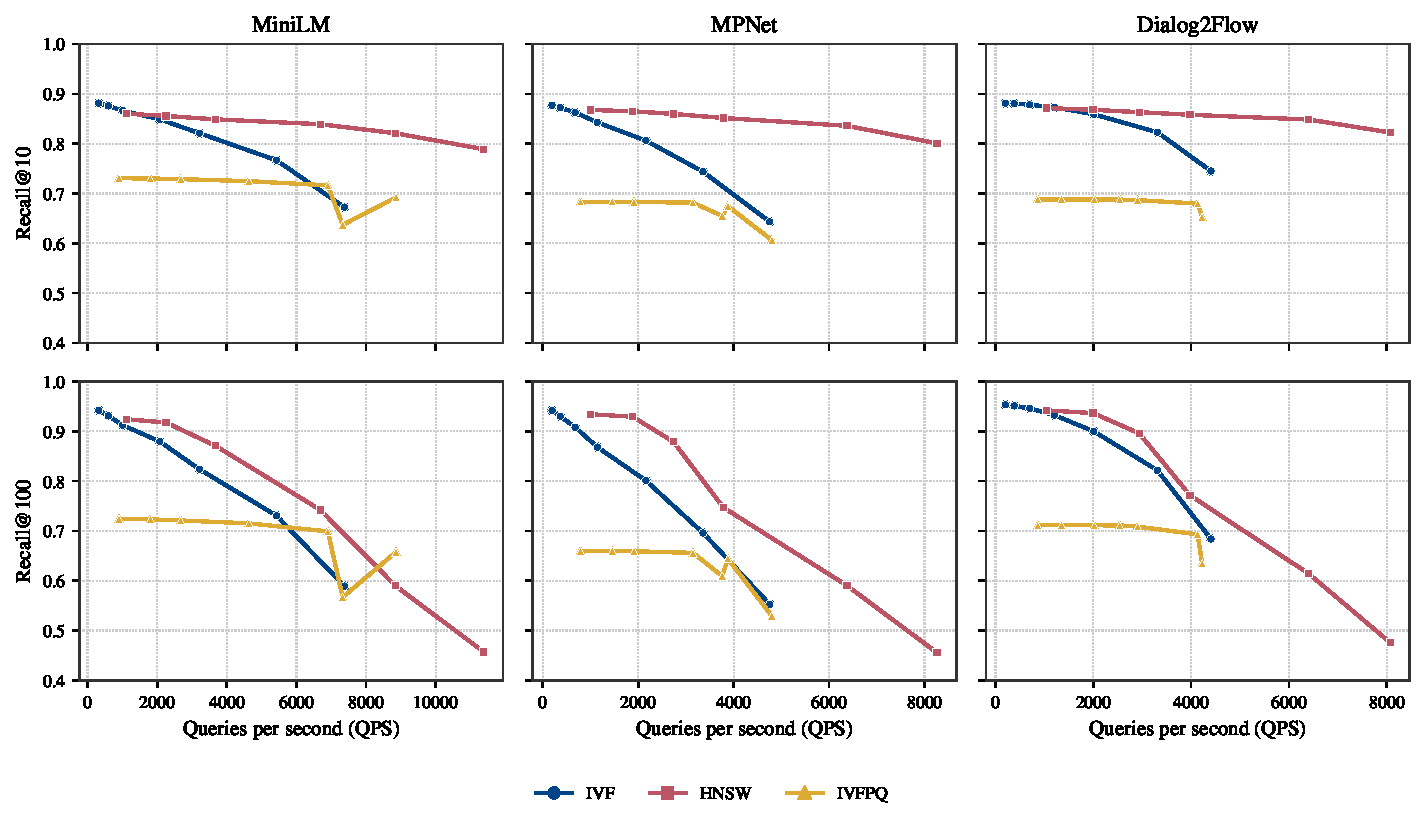
\includegraphics[width=\textwidth]{figures/fig_recall10_recall100_qps_embeddings_independientes.pdf}
\caption{Curvas Recall@10 y Recall@100 versus QPS para embeddings estáticos.}
\label{fig:recall_qps_static}
\end{figure}

La Tabla~\ref{tab:static_representative} resume configuraciones representativas de alta recuperación para \textit{IVF} y \textit{HNSW}, junto con la referencia exacta \textit{FlatL2} y una configuración comprimida mediante \textit{IVFPQ}.  

\begin{table}[ht]
\centering
\small
\setlength{\tabcolsep}{4pt}
\caption{Resultados de recuperación aproximada sobre representaciones estáticas.}
\label{tab:static_representative}
\begin{tabular}{llrrrrr}
\toprule
Representación & Índice/config. & R@1 & R@10 & R@100 & QPS & Mem. (MB) \\
\midrule
\textit{MiniLM} & \textit{FlatL2} & 1.000 & 1.000 & 1.000 & 62 & 1450.2 \\
\textit{MiniLM} & \textit{IVF} $nprobe=64$ & 0.692 & \textbf{0.881} & \textbf{0.942} & 320 & 1463.8 \\
\textit{MiniLM} & \textit{HNSW} $efSearch=256$ & 0.674 & 0.860 & 0.924 & \textbf{1115} & 1691.9 \\
\textit{MiniLM} & \textit{IVFPQ} $nprobe=64$ & 0.757 & 0.731 & 0.724 & 900 & \textbf{44.1} \\
\midrule
\textit{MPNet} & \textit{FlatL2} & 1.000 & 1.000 & 1.000 & 32 & 2900.5 \\
\textit{MPNet} & \textit{IVF} $nprobe=64$ & 0.668 & \textbf{0.877} & \textbf{0.942} & 195 & 2920.0 \\
\textit{MPNet} & \textit{HNSW} $efSearch=256$ & 0.660 & 0.868 & 0.934 & \textbf{1001} & 3142.2 \\
\textit{MPNet} & \textit{IVFPQ} $nprobe=64$ & 0.730 & 0.683 & 0.660 & 791 & \textbf{50.5} \\
\midrule
\textit{Dialog2Flow} & \textit{FlatL2} & 1.000 & 1.000 & 1.000 & 34 & 2900.5 \\
\textit{Dialog2Flow} & \textit{IVF} $nprobe=64$ & 0.685 & \textbf{0.881} & \textbf{0.953} & 203 & 2920.0 \\
\textit{Dialog2Flow} & \textit{HNSW} $efSearch=256$ & 0.676 & 0.872 & 0.942 & \textbf{1041} & 3142.2 \\
\textit{Dialog2Flow} & \textit{IVFPQ} $nprobe=64$ & 0.730 & 0.688 & 0.711 & 865 & \textbf{50.5} \\
\bottomrule
\end{tabular}
\end{table}

Los resultados muestran que \textit{dialog2flow-joint-bert-base} mantiene un comportamiento competitivo frente a los modelos generales de \textit{sentence embeddings}, lo que indica que un espacio específico para flujos conversacionales puede indexarse eficientemente mediante métodos ANN sin degradar de manera sustancial el compromiso entre recuperación y velocidad. El patrón Recall@1 > Recall@10 > Recall@100 de IVFPQ, contraintuitivo a primera vista, surge porque Recall@k (intersección de los $k$ vecinos aproximados y exactos dividida por $k$) no es monótona en $k$ y los turnos casi idénticos de los corpus TOD caen fuera de la intersección.

Una segunda etapa experimental exploró el efecto de las variantes acumulativas normalizadas sobre la geometría de los espacios vectoriales. La Tabla~\ref{tab:accumulative_geometry} compara cada representación estática con su variante acumulativa mediante la similitud coseno promedio y mediana entre \(e_t\) y \(h_t\), junto con la superposición de vecinos exactos entre ambos espacios, permitiendo observar en qué medida la acumulación modifica la estructura local de cada \textit{embedding} base.

\begin{table}[ht]
\centering
\small
\setlength{\tabcolsep}{5pt}
\caption{Comparación geométrica entre representaciones estáticas y acumulativas.}
\label{tab:accumulative_geometry}
\begin{tabular}{lrrrrr}
\toprule
Base & Sim. media & Sim. mediana & Overlap@1 & Overlap@10 & Overlap@100 \\
\midrule
\textit{MiniLM} & 0.412 & 0.344 & 0.256 & 0.100 & 0.035 \\
\textit{MPNet} & 0.405 & 0.345 & 0.240 & 0.097 & 0.032 \\
\textit{Dialog2Flow} & \textbf{0.727} & \textbf{0.702} & \textbf{0.296} & \textbf{0.175} & \textbf{0.152} \\
\bottomrule
\end{tabular}
\end{table}

Los resultados muestran que el efecto de la acumulación no es uniforme entre representaciones. En \textit{MiniLM} y \textit{MPNet}, la similitud entre la representación estática y la acumulativa se ubica alrededor de 0.41, con valores de Overlap@100 cercanos a 0.03, lo que indica una modificación sustantiva de la vecindad local. En cambio, sobre \textit{Dialog2Flow} la similitud promedio alcanza 0.727 y el Overlap@100 aumenta a 0.152, sugiriendo una mayor estabilidad geométrica frente a la acumulación secuencial.

Para complementar esta lectura, la Figura~\ref{fig:dialog2flow_accumulative} explora el espacio \textit{Dialog2Flow}, seleccionado por su carácter específico para flujos conversacionales y por su comportamiento competitivo en la evaluación ANN inicial.

\begin{figure}[ht]
\centering
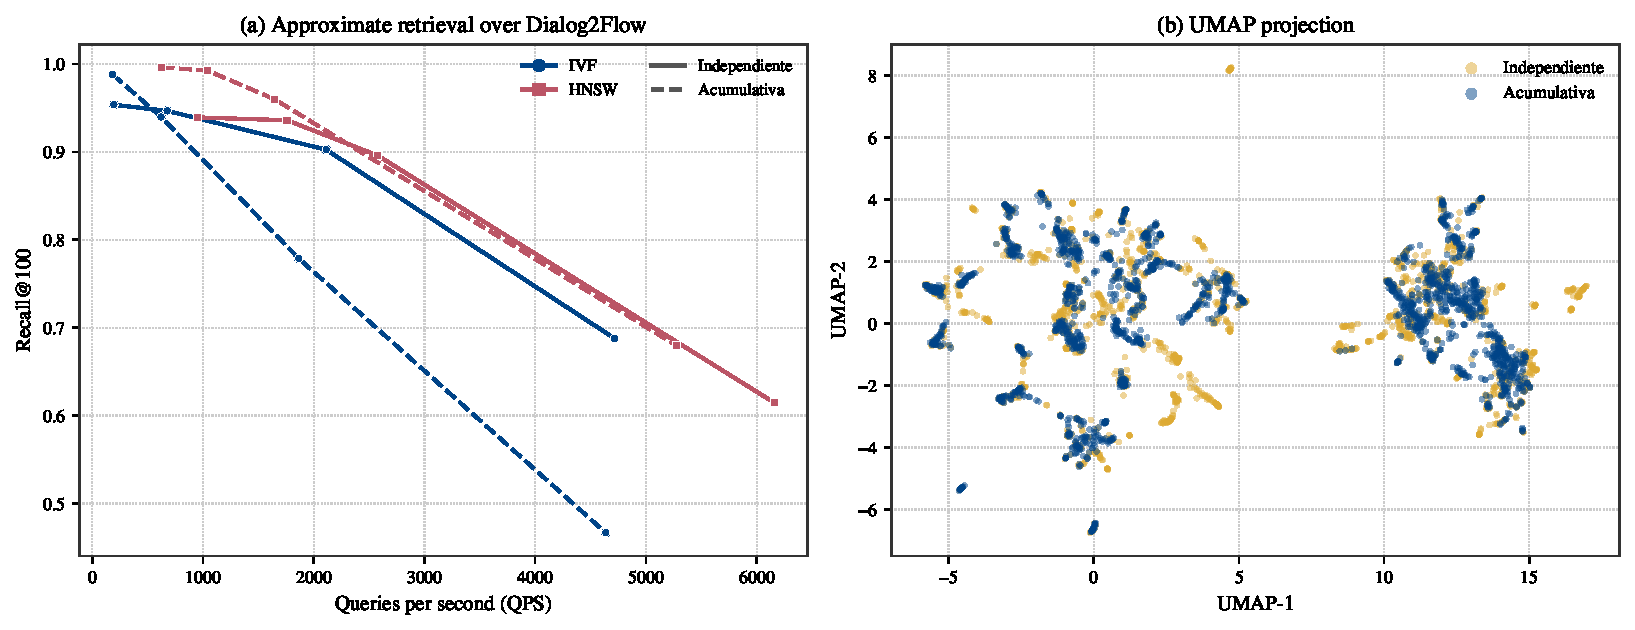
\includegraphics[width=\textwidth]{figures/fig_dialog2flow_independiente_vs_acumulativa_1x2.pdf}
\caption{Análisis exploratorio sobre el espacio \textit{Dialog2Flow}.}
\label{fig:dialog2flow_accumulative}
\end{figure}

La Figura~\ref{fig:dialog2flow_accumulative} complementa el análisis geométrico anterior mediante dos vistas del espacio \textit{Dialog2Flow}. En el panel izquierdo, las curvas Recall@100 versus QPS muestran que la variante acumulativa alcanza valores superiores de recuperación respecto de la representación estática, tanto en \textit{IVF} como en \textit{HNSW}, especialmente en configuraciones de mayor exploración. Este comportamiento sugiere que la acumulación secuencial no sólo modifica la representación, sino que puede inducir una geometría más favorable para la búsqueda aproximada. En el panel derecho, la proyección UMAP evidencia una reorganización visible del espacio, consistente con la baja superposición parcial observada entre vecindades estáticas y acumulativas.


En este sentido, la tercera etapa experimental tuvo como objetivo analizar si las diferencias geométricas observadas se reflejan en vecindades semántico-funcionalmente más plausibles. Para ello, se aplicó el protocolo asistido por LLM\footnote{Como modelo juez se utilizó \texttt{gpt-4.1-mini} (temperatura $0$), evaluando $|Q|=100$ consultas por configuración evaluada; cada vecino del top-10 recibió un puntaje ordinal en escala 1--5 y MSS@10 se computa sobre la similitud global. El \textit{prompt}, el esquema de salida y los puntajes se documentan en el repositorio público del trabajo.} definido en la Sección~\ref{sec:methodology}, calculando MSS@10 para cada combinación de representación, variante e índice ANN.

\begin{table}[ht]
\centering
\small
\setlength{\tabcolsep}{5pt}
\caption{Evaluación semántico-funcional de vecinos recuperados. Se reporta MSS@10 junto con el desvío estándar entre consultas.}
\label{tab:mss_semantic_eval}
\begin{tabular}{llrrr}
\toprule
Representación & Variante & IVF & HNSW & IVFPQ \\
\midrule
\textit{MiniLM} & Estática & 3.399 $\pm$ 0.758 & 3.416 $\pm$ 0.741 & 3.346 $\pm$ 0.803 \\
\textit{MiniLM} & Acumulativa & 3.315 $\pm$ 0.754 & 3.334 $\pm$ 0.758 & 3.234 $\pm$ 0.769 \\
\midrule
\textit{MPNet} & Estática & 3.381 $\pm$ 0.773 & 3.358 $\pm$ 0.803 & 3.368 $\pm$ 0.819 \\
\textit{MPNet} & Acumulativa & 3.309 $\pm$ 0.776 & 3.310 $\pm$ 0.761 & 3.197 $\pm$ 0.742 \\
\midrule
\textit{Dialog2Flow} & Estática & 3.401 $\pm$ 0.759 & 3.377 $\pm$ 0.757 & 3.315 $\pm$ 0.825 \\
\textit{Dialog2Flow} & Acumulativa & \textbf{3.672 $\pm$ 0.647} & \textbf{3.664 $\pm$ 0.643} & \textbf{3.593 $\pm$ 0.707} \\
\bottomrule
\end{tabular}
\end{table}

La Tabla~\ref{tab:mss_semantic_eval} muestra que la variante acumulativa alcanza sus mejores resultados cuando se aplica sobre \textit{Dialog2Flow}. En los tres índices ANN evaluados, \textit{Dialog2Flow} acumulativo obtiene los valores más altos de MSS@10, con puntajes entre 3.59 y 3.67 sobre una escala de 1 a 5. En contraste, la acumulación sobre los modelos generales \textit{MiniLM} y \textit{MPNet} no produce una mejora equivalente: sus variantes acumulativas presentan valores levemente inferiores a las representaciones estáticas en los tres índices.

Para analizar si la mejora de \textit{Dialog2Flow} acumulativo dependía de pocos casos extremos, se realizó una comparación pareada por consulta entre las variantes estática y acumulativa. La Tabla~\ref{tab:paired_semantic_eval} reporta el porcentaje de consultas en las que la variante acumulativa obtuvo un valor de SS@10 superior al de la variante estática.

\begin{table}[ht]
\centering
\small
\setlength{\tabcolsep}{6pt}
\caption{Porcentaje de consultas en las que la variante acumulativa supera a la estática según SS@10.}
\label{tab:paired_semantic_eval}
\begin{tabular}{lrrr}
\toprule
Representación & IVF & HNSW & IVFPQ \\
\midrule
\textit{MiniLM} & 47\% & 48\% & 44\% \\
\textit{MPNet} & 48\% & 48\% & 41\% \\
\textit{Dialog2Flow} & \textbf{63\%} & \textbf{67\%} & \textbf{57\%} \\
\bottomrule
\end{tabular}
\end{table}

La comparación pareada refuerza la interpretación anterior. En \textit{Dialog2Flow}, la variante acumulativa supera a la estática en la mayoría de las consultas para los tres índices evaluados, especialmente en \textit{HNSW} e \textit{IVF}. En cambio, para \textit{MiniLM} y \textit{MPNet}, los porcentajes se mantienen cercanos al equilibrio o por debajo del 50\%. Esto sugiere que la mejora observada en \textit{Dialog2Flow} no depende sólo de valores extremos, sino que se distribuye sobre una proporción mayoritaria de consultas.

En conjunto, estos resultados indican que la acumulación secuencial normalizada no constituye una mejora universal sobre cualquier espacio de \textit{embeddings}. Su efecto depende del espacio base: en los modelos generales modifica la vecindad sin mejorar su plausibilidad semántico-funcional, mientras que en \textit{Dialog2Flow} induce vecindades más favorables tanto desde el punto de vista geométrico como semántico-funcional.

\begin{table}[ht]
\centering
\caption{Comparación de las variantes EMA de Dialog2Flow frente al mejor resultado dinámico previo. Se reporta MSS@10 para cada índice ANN. La última columna indica la diferencia entre el mejor resultado obtenido por cada valor de $\alpha$ y el mejor baseline dinámico previo ($\mathrm{MSS@10}=3.665$).}
\label{tab:ema_alpha_vs_dynamic_d2f}
\begin{tabular}{lccccc}
\toprule
\textbf{Representación} & $\boldsymbol{\alpha}$ & \textbf{IVF} & \textbf{HNSW} & \textbf{IVFPQ} & $\boldsymbol{\Delta}$ \textbf{vs. dinámico} \\
\midrule
D2F dinámico previo & --  & \textbf{3.665} & 3.661 & 3.647 & 0.000 \\
\midrule
D2F-EMA & 0.1 & 3.180 & 3.203 & 3.181 & -0.462 \\
D2F-EMA & 0.2 & 3.260 & 3.237 & 3.326 & -0.339 \\
D2F-EMA & 0.3 & 3.392 & 3.387 & 3.454 & -0.211 \\
D2F-EMA & 0.4 & 3.582 & 3.577 & 3.565 & -0.083 \\
D2F-EMA & 0.5 & 3.671 & 3.661 & 3.640 & +0.006 \\
D2F-EMA & \textbf{0.6} & \textbf{3.797} & \textbf{3.776} & \textbf{3.714} & \textbf{+0.132} \\
D2F-EMA & 0.7 & 3.755 & 3.758 & 3.702 & +0.093 \\
D2F-EMA & 0.8 & 3.652 & 3.639 & 3.575 & -0.013 \\
D2F-EMA & 0.9 & 3.431 & 3.414 & 3.491 & -0.174 \\
\bottomrule
\end{tabular}
\end{table}

\begin{figure}[ht]
\centering
\includegraphics[width=\textwidth]{figures/visual-ema.png}
\caption{Recall@10 and Recall@100 versus QPS curves for static embeddings.}
\label{fig:recall_qps_static}
\end{figure}


\section{Conclusiones y trabajo futuro}
\label{sec:conclusions}

En este trabajo se estudió la búsqueda aproximada de vecinos sobre \textit{embeddings} estáticos y acumulativos para memoria conversacional en diálogos orientados a tareas. A partir de una colección de 101.021 diálogos y 1.000.023 turnos derivados de \textit{Dialog2Flow}, se evaluaron tres espacios de representación y los índices \textit{IVF}, \textit{HNSW} e \textit{IVFPQ} implementados en \textit{FAISS}.

Los resultados muestran que los métodos ANN permiten recuperar representaciones conversacionales a escala con compromisos controlables entre \textit{recall}, QPS y memoria. \textit{HNSW} presentó un balance favorable entre recuperación y velocidad, mientras que \textit{IVFPQ} redujo sustancialmente la memoria a costa de una pérdida de \textit{recall}.

El aporte principal surge al comparar representaciones estáticas y acumulativas. La mejora asociada a la acumulación secuencial se concentró en \textit{Dialog2Flow}: aplicada sobre este espacio, produjo vecindades más favorables tanto desde el punto de vista geométrico como semántico-funcional, obtuvo los mayores valores de MSS@10 bajo \textit{IVF}, \textit{HNSW} e \textit{IVFPQ}, y superó a su variante estática en la mayoría de las consultas evaluadas. En los modelos generales \textit{MiniLM} y \textit{MPNet}, no se observó una mejora equivalente.

Estos resultados sugieren que la utilidad de las representaciones acumulativas depende de la geometría del espacio base. Una acumulación simple puede no ser suficiente sobre \textit{embeddings} generales, pero resulta prometedora cuando se aplica sobre espacios orientados a regularidades de flujos conversacionales.

Como trabajo futuro, se propone explorar políticas acumulativas más expresivas, incorporando ponderación temporal, distinción entre hablantes, actos de diálogo, \textit{slots} e intenciones. También resulta relevante evaluar estas representaciones en tareas concretas de diálogo orientado a tareas, como selección de próxima acción, detección de información faltante o recomendación de trayectorias conversacionales.

\bibliographystyle{splncs04}
\bibliography{References}

\end{document}